\section{Infrastructure de traitement}
La structure interne des systèmes de gestions de flux de données diffère entre les implémentations. Toutefois, plusieurs concepts fondateurs sont couramment utilisés pour permettre l'exécution correcte des requêtes ou pour permettre la gestion des multi-échelles.
\TODO{PLAN}
\subsection{Du modèle vers l'implémentation}
Le modèle théorique permet de savoir la sémantique exacte des expressions de requêtes. La mise en œuvre de ces expressions est plus délicate. La connaissance de cette structure est nécessaire non seulement pour comprendre le fonctionnement des SGFD. Mais de plus, cela permet la mise en œuvre de solutions de médiations de systèmes~\cite{Tatbul:integration}.

\subsubsection{Les résultats intermédiaires}
Comme présenté précédemment en section~\ref{sec:rw:supervision:datastream}, la gestion de flux de données se décompose en trois composants principaux : les sources, les opérateurs et les puits. Les opérateurs consomment une ou plusieurs entités (un flux par exemple) et produisent une nouvelle entité. Ces entités sont matérialisés par des résultats intermédiaires en implémentation comme présenté dans la figure~\ref{fig:rw:sgfd:modeleimplem}.
\begin{figure}
    \centering
    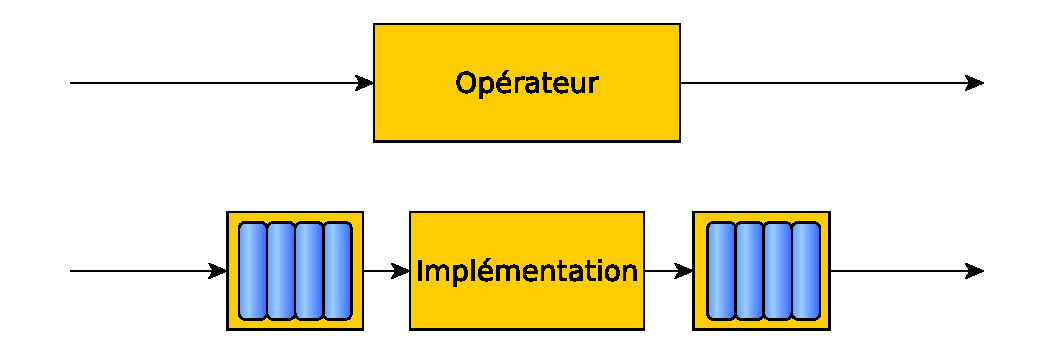
\includegraphics[width=0.8\textwidth]{rw-sgfd-modeleimplem}
    \caption{Implémentation d'un opérateur avec les résultats intermédiaires}\label{fig:rw:sgfd:modeleimplem}
\end{figure}

Ces résultats intermédiaires utilisent des mémoires tampons (et occasionnellement des supports persistants~\cite{Abadi:aurora}). Ces résultats sont manipulé par une interface d'appel très simple en général basé sur les primitives \textit{push} et \textit{pop} tel une pile. Le point crucial de la gestion de flux de données est de maîtriser ces canaux. Leur fonctionnement peut toutefois être plus compliqué en introduisant des primitives d'ordres ou de sélection comme dans les \textit{SweepArea} de \textit{PIPES}~\cite{Kramer:semantics}.

\subsubsection{L'exécution}
Deux types d'exécutions sont référencés : les non-bloquantes et les  bloquantes~\cite{Babcock:issues}. Originellement, un opérateur \textit{bloquant} est \enquote{\it un opérateur qui n'est pas capable de produire son premier n-uplet tant que l'ensemble de son entrée n'a pas été consommé}. Les opérateurs souvent cités sont les agrégats. Par la suite, grâce aux recherches sur les fenêtres~\cite{Maier:semantics}, le terme est généralisé aux opérations de fenêtrages dont le décalage est différent de \textit{1 n-uplet}.

Un opérateur non-bloquant a pour objectif de vider le plus rapidement possible les canaux. Un opérateur bloquant lui attendra.


\subsection{Passage à l'échelle}
